\documentclass[letterpaper]{article}
\usepackage[submission]{aaai2027}
\usepackage[hyphens]{url}
\usepackage{graphicx}
\urlstyle{rm}
\def\UrlFont{\rm}
\usepackage{natbib}
\frenchspacing

\usepackage{amsmath}
\usepackage{amssymb}
\usepackage{booktabs}
\usepackage{multirow}
\usepackage{float}
\usepackage{algorithm}
\usepackage{algorithmic}
\usepackage{tikz}
\usetikzlibrary{shapes.geometric, arrows.meta, positioning, fit, calc, backgrounds}

% Resolve references to the supplementary material (appendices and S-tables).
% \bibcite is suppressed so the imported .aux does not clash with the local
% bibliography.
\usepackage{xr}
\makeatletter
\begingroup
\let\bibcite\@gobbletwo
\externaldocument{supplementary}
\endgroup
\makeatother

\pdfinfo{
/Title (Infrastructure-Aware Wildfire Coordination: A Benchmark on Validated Fire-Spread Physics and a Value-Aware Hierarchical Multi-Agent Baseline)
/Author (Anonymous)
/TemplateVersion (2027.1)
}

\setcounter{secnumdepth}{2}

\title{Infrastructure-Aware Wildfire Coordination: \\ A Benchmark on Validated Fire-Spread Physics and a \\ Value-Aware Hierarchical Multi-Agent Baseline}
\author{Anonymous Authors}
\affiliations{Anonymous Affiliations}

\begin{document}
\maketitle

% ====================================================================
% ABSTRACT
% ====================================================================
\begin{abstract}
Defending critical infrastructure during a wildfire is a prioritization problem before it is a suppression problem: with limited crews and an advancing front, the question is which assets to save. We contribute an infrastructure-aware coordination benchmark and a reference method, together with a negative result that we believe is the more durable finding. The benchmark couples the validated Cell2Fire spread engine to a multi-agent suppression wrapper, under a fixed five-seed protocol, over two GIS-derived landscapes whose asset geometries contrast sharply: concentrated Saudi petroleum infrastructure against a scattered California wildland-urban interface. The reference method, \textbf{HiVA}, pairs a rule-based value-aware commander with a tactical policy trained by imitation and refined by proximal policy optimization (PPO). HiVA attains the lowest Weighted Economic Loss and the highest Infrastructure Survival Rate in both regions, but after Holm correction its advantage over flat multi-agent reinforcement learning (MARL) holds on California only; on Saudi it falls within seed variance, and a supervision-matched component analysis shows that expert demonstrations, not the hierarchy, supply most of that gap. Explicit inter-agent communication contributes nothing measurable at three agents. Off distribution the picture reverses: a value-blind nearest-frontier heuristic attains the larger protective margin in five of six perturbed conditions and beats transferred HiVA in both cross-region directions. We therefore state the main claim as a tradeoff: learned value-awareness buys in-distribution prioritization at the cost of geometric generalization. We release the benchmark, code, checkpoints, GIS pipeline, and hashed manifests.
\end{abstract}

% ====================================================================
% 1. INTRODUCTION
% ====================================================================
\section{Introduction}
\label{sec:intro}

Wildfire suppression is a resource-allocation problem played out on a moving hazard. When petroleum refineries, pipeline junctions, or residential structures sit in the path of an advancing front, minimizing total burned area stops being the right objective: crews must decide which assets are worth defending and accept that others will burn. That triage framing, rather than containment for its own sake, separates infrastructure defense from generic fire suppression, and it is what this paper studies.

\paragraph{Prioritization under partial observability.} An agent with a local, egocentric view cannot see the distant refinery it is supposed to protect. Flat decentralized multi-agent reinforcement learning (MARL) policies such as MAPPO~\citep{yu2022mappo} and QMIX~\citep{rashid2018qmix} optimize against what they can see, which in practice means the nearest flames. A temporal decomposition is the natural response: a slow strategic layer that assigns agents to threatened high-value assets, and a fast tactical layer that executes suppression. Our reference method, \textbf{HiVA} (Hierarchical Value-Aware coordination), is built on that split, with a commander that dispatches agents by threat-weighted asset value and a learned tactical policy refined by reinforcement learning (RL).

\paragraph{What we claim, and what we do not.} We claim no algorithmic novelty. Every component of HiVA is standard: a hand-written assignment rule, a convolutional actor with mean-pooled messages, behavior cloning, and PPO. The contribution is the benchmark and the analysis it makes possible, with HiVA as a transparent reference point. That framing obliges precision about attribution, and precision cuts against us: given the same expert demonstrations, learned baselines largely dissolve HiVA's Saudi advantage, so demonstrations, not hierarchy, carry that region.

\paragraph{The negative result is the finding.} Our most robust observation is not that HiVA wins. It is that a value-blind reactive heuristic, with no notion of asset value at all, generalizes better in five of the six perturbed conditions we tested and beats transferred HiVA in both cross-region directions. Read with the in-distribution results, this supports a falsifiable claim: value-aware prioritization is worth its complexity near the training distribution and becomes a liability away from it.

\paragraph{Contributions.}
\begin{enumerate}\itemsep0pt
    \item An \textbf{infrastructure-aware coordination benchmark} on Cell2Fire~\citep{pais2021cell2fire} with two landscapes derived from public geographic information system (GIS) data, a released data pipeline, hashed manifests, and an explicit accounting (Appendix~\ref{app:simulator}) of which dynamics are validated fire physics and which are our wrapper.
    \item \textbf{HiVA}, a value-aware hierarchical reference system composing a rule-based assignment, a tactical actor, behavior cloning, and PPO fine-tuning. It attains the best mean Weighted Economic Loss (WEL) and Infrastructure Survival Rate (ISR) in both regions; after multiplicity correction its improvement over the strongest flat baseline holds on California and not on Saudi.
    \item A \textbf{supervision-matched component analysis} separating three explanations for the gains: the value-aware hierarchy, expert demonstrations, and RL refinement. Message passing is not among them at three agents, and we report the scale at which that null breaks.
    \item A \textbf{robustness and transfer analysis} whose headline is negative: under held-out ignitions, rotated wind, rotated asset layouts, and cross-region transfer, value-blind reactive coverage attains the larger $\Delta$WEL in five of six perturbed conditions and wins both transfer directions.
\end{enumerate}

% ====================================================================
% 2. RELATED WORK
% ====================================================================
\section{Related Work}
\label{sec:related}

\paragraph{Wildfire simulation and GIS-based planning.} Fire-spread modeling has moved from cellular automata toward physically grounded simulators. Cell2Fire~\citep{pais2021cell2fire} implements the Canadian Forest Fire Behavior Prediction (FBP) system with heterogeneous fuels, wind, and slope corrections, and is the spread engine we build on. Operations research remains the deployed state of the art for suppression \emph{planning}, optimizing firebreak or resource placement by mixed-integer programming~\citep{hu2009wildfire}; those methods assume global observability and quasi-static fire, so they complement the sequential, partially observed setting studied here. We nonetheless include a myopic dispatch baseline, because a dispatch rule is what fire agencies actually run.

\paragraph{Reinforcement learning for wildfire.} Prior RL work covers detection from unmanned aerial vehicles~\citep{ghali2022}, landscape-scale fuel treatment~\citep{altamimi2022wildfire}, and grid-based suppression on Cell2Fire~\citep{shen2022firehose}. Firehose~\citep{shen2022firehose} is closest in setup, although it is single-agent, optimizes burned area alone, and is an unrefereed report. Multi-agent wildfire environments have grown since, covering joint perception-action tasks (FireCommander,~\citealp{seraj2020firecommander}), Unity-based aerial suppression with a public leaderboard (HIVEX,~\citealp{siedler2025hivex}), agent and task openness (MOASEI,~\citealp{patino2025moasei}), and large-scale agentic coordination with heterogeneous crews (CREW-Wildfire,~\citealp{hyun2025crewwildfire}).

We therefore scope our claim narrowly. We are not first to study multi-agent wildfire suppression or to release a wildfire benchmark; what is distinctive is a conjunction of three properties: an \emph{asset-value-weighted} objective rather than burned area or containment time, spread dynamics from a \emph{validated} FBP implementation rather than a bespoke automaton, and landscapes derived from documented public GIS sources. HIVEX and CREW-Wildfire use custom spread models and score containment or task success; MOASEI's wildfire track scores expected utility under openness rather than infrastructure value.

\paragraph{Cooperative MARL and communication.} Centralized training with decentralized execution dominates cooperative MARL: QMIX~\citep{rashid2018qmix} factorizes joint values under monotonicity, MAPPO~\citep{yu2022mappo} pairs PPO~\citep{schulman2017} with a centralized critic, and CommNet~\citep{sukhbaatar2016learning} and TarMAC~\citep{das2019tarmac} add learned messaging. The communication literature has been surveyed along nine design dimensions~\citep{zhu2024commsurvey}, which scopes our null: our architecture sits at the simplest point of that space (broadcast, mean-pooled, unconditioned), so our finding bounds that corner only.

\paragraph{Hierarchical RL, imitation, and fine-tuning.} Options~\citep{sutton1999options}, feudal networks~\citep{vezhnevets2017feudal}, hierarchies of machines~\citep{parr1997hams}, and MAXQ~\citep{dietterich1998maxq} established temporal and subtask abstraction; in multi-agent settings RODE~\citep{wang2021rode} decomposes by role, MAVEN~\citep{mahajan2019maven} by shared latents, and HAVEN~\citep{xu2023haven} across levels and agents simultaneously. Most of this work optimizes both levels jointly, whereas we freeze a transparent rule at the strategic level and learn only the tactical one. Combining imitation with RL is likewise established, through DAgger~\citep{ross2011reduction}, cloning followed by RL~\citep{silver2016mastering, rajeswaran2018learning}, and KL-regularized fine-tuning~\citep{wu2019behavior}. Section~\ref{sec:ablation} gives baselines the same imitation head start, which matters more than the hierarchy on one of our landscapes.

% ====================================================================
% 3. PROBLEM FORMULATION
% ====================================================================
\section{Problem Formulation}
\label{sec:formulation}

We model infrastructure-aware suppression as a decentralized partially observable Markov decision process (Dec-POMDP) extended with temporal abstraction.

\paragraph{State.} The global state $s = \langle S_{\text{fire}}, S_{\text{asset}}, S_{\text{agent}} \rangle$ comprises a binary active-fire grid $S_{\text{fire}} \in \{0,1\}^{H \times W}$ evolved by Cell2Fire, an infrastructure criticality map $S_{\text{asset}} \in \mathbb{R}_{\geq 0}^{H \times W}$, and agent positions $S_{\text{agent}} = \{(y_i, x_i)\}_{i=1}^N$.

\paragraph{Observations.} Each agent observes an egocentric $C \times C$ crop ($C = 9$) with eight channels: five spatial crops (active fire, treated cells, fuel type, criticality, teammate occupancy), one homogeneous channel carrying the global burning fraction, and two carrying the normalized offset $\bigl((y_i^*-y_i)/H,\ (x_i^*-x_i)/W\bigr)$ to the agent's strategic target. Agents never see the full grid. The burning-fraction channel deliberately relaxes strict decentralization: it stands in for the situational awareness a real crew receives by radio, but it is in tension with the Dec-POMDP framing and we flag it as such. The observation \emph{space} is identical across methods. Under HiVA the last two channels point to the assigned asset; for flat baselines, which issue no assignments, they encode displacement from the spawn location and are nearly uninformative. Section~\ref{sec:setup} therefore adds a value-aware flat baseline receiving a target signal without any hierarchy, so ``hierarchy'' is not confounded with ``access to asset information.''

\paragraph{Actions.} Every $T_{\text{macro}} = 10$ steps, each agent receives a strategic target: a high-value threatened asset to defend. At every environment step it executes a micro-action $a_i^t \in \{$stay, up, down, left, right, treat$\}$.

\paragraph{Reward.} The suppression objective rewards protecting economic value. Let $\text{WEL} = \sum_j v_j \cdot \mathbf{1}[\text{asset}_j \text{ burned}]$ denote the Weighted Economic Loss and $\text{ISR}$ the fraction of assets surviving. The per-step reward is
\begin{equation}
\label{eq:reward}
\begin{split}
r_t = {}& -\Delta \text{WEL}_t - (\kappa-1)\,\Delta \text{WEL}^{\text{crit}}_t \\
        & + \alpha\, \Delta \text{ISR}_t + \eta\,\bigl(b_{t-1} - b_t\bigr) - \lambda\, c_t ,
\end{split}
\end{equation}
where $b_t$ counts burning cells, $c_t$ counts agent pairs occupying the same cell, $\alpha = 20$ upweights survival, $\eta = 0.05$ is a light firebreak-shaping coefficient, $\lambda = 0.1$ is a coordination penalty discouraging redundant co-location, and $\kappa = 2.0$ is the catastrophe weight applied to the subset $\text{WEL}^{\text{crit}}$ of loss on assets above the criticality threshold. The episode return used for evaluation reduces to WEL and ISR alone; the remaining terms shape training only. Appendix~\ref{app:hyperparameters} reports sensitivity to $\alpha$ and $\eta$.

% ====================================================================
% 4. METHOD
% ====================================================================
\section{The HiVA Reference System}
\label{sec:method}

HiVA splits infrastructure defense into a value-aware strategic layer and a learned tactical layer (Figure~\ref{fig:architecture}). Every $T_{\text{macro}} = 10$ steps, a commander assigns each agent a threatened high-value asset; between assignments a tactical policy selects micro-actions that build the firebreak protecting it. That policy is warm-started by behavior cloning (BC) and refined by proximal policy optimization (PPO)~\citep{schulman2017} on Equation~\ref{eq:reward}.

\begin{figure*}[t]
\centering
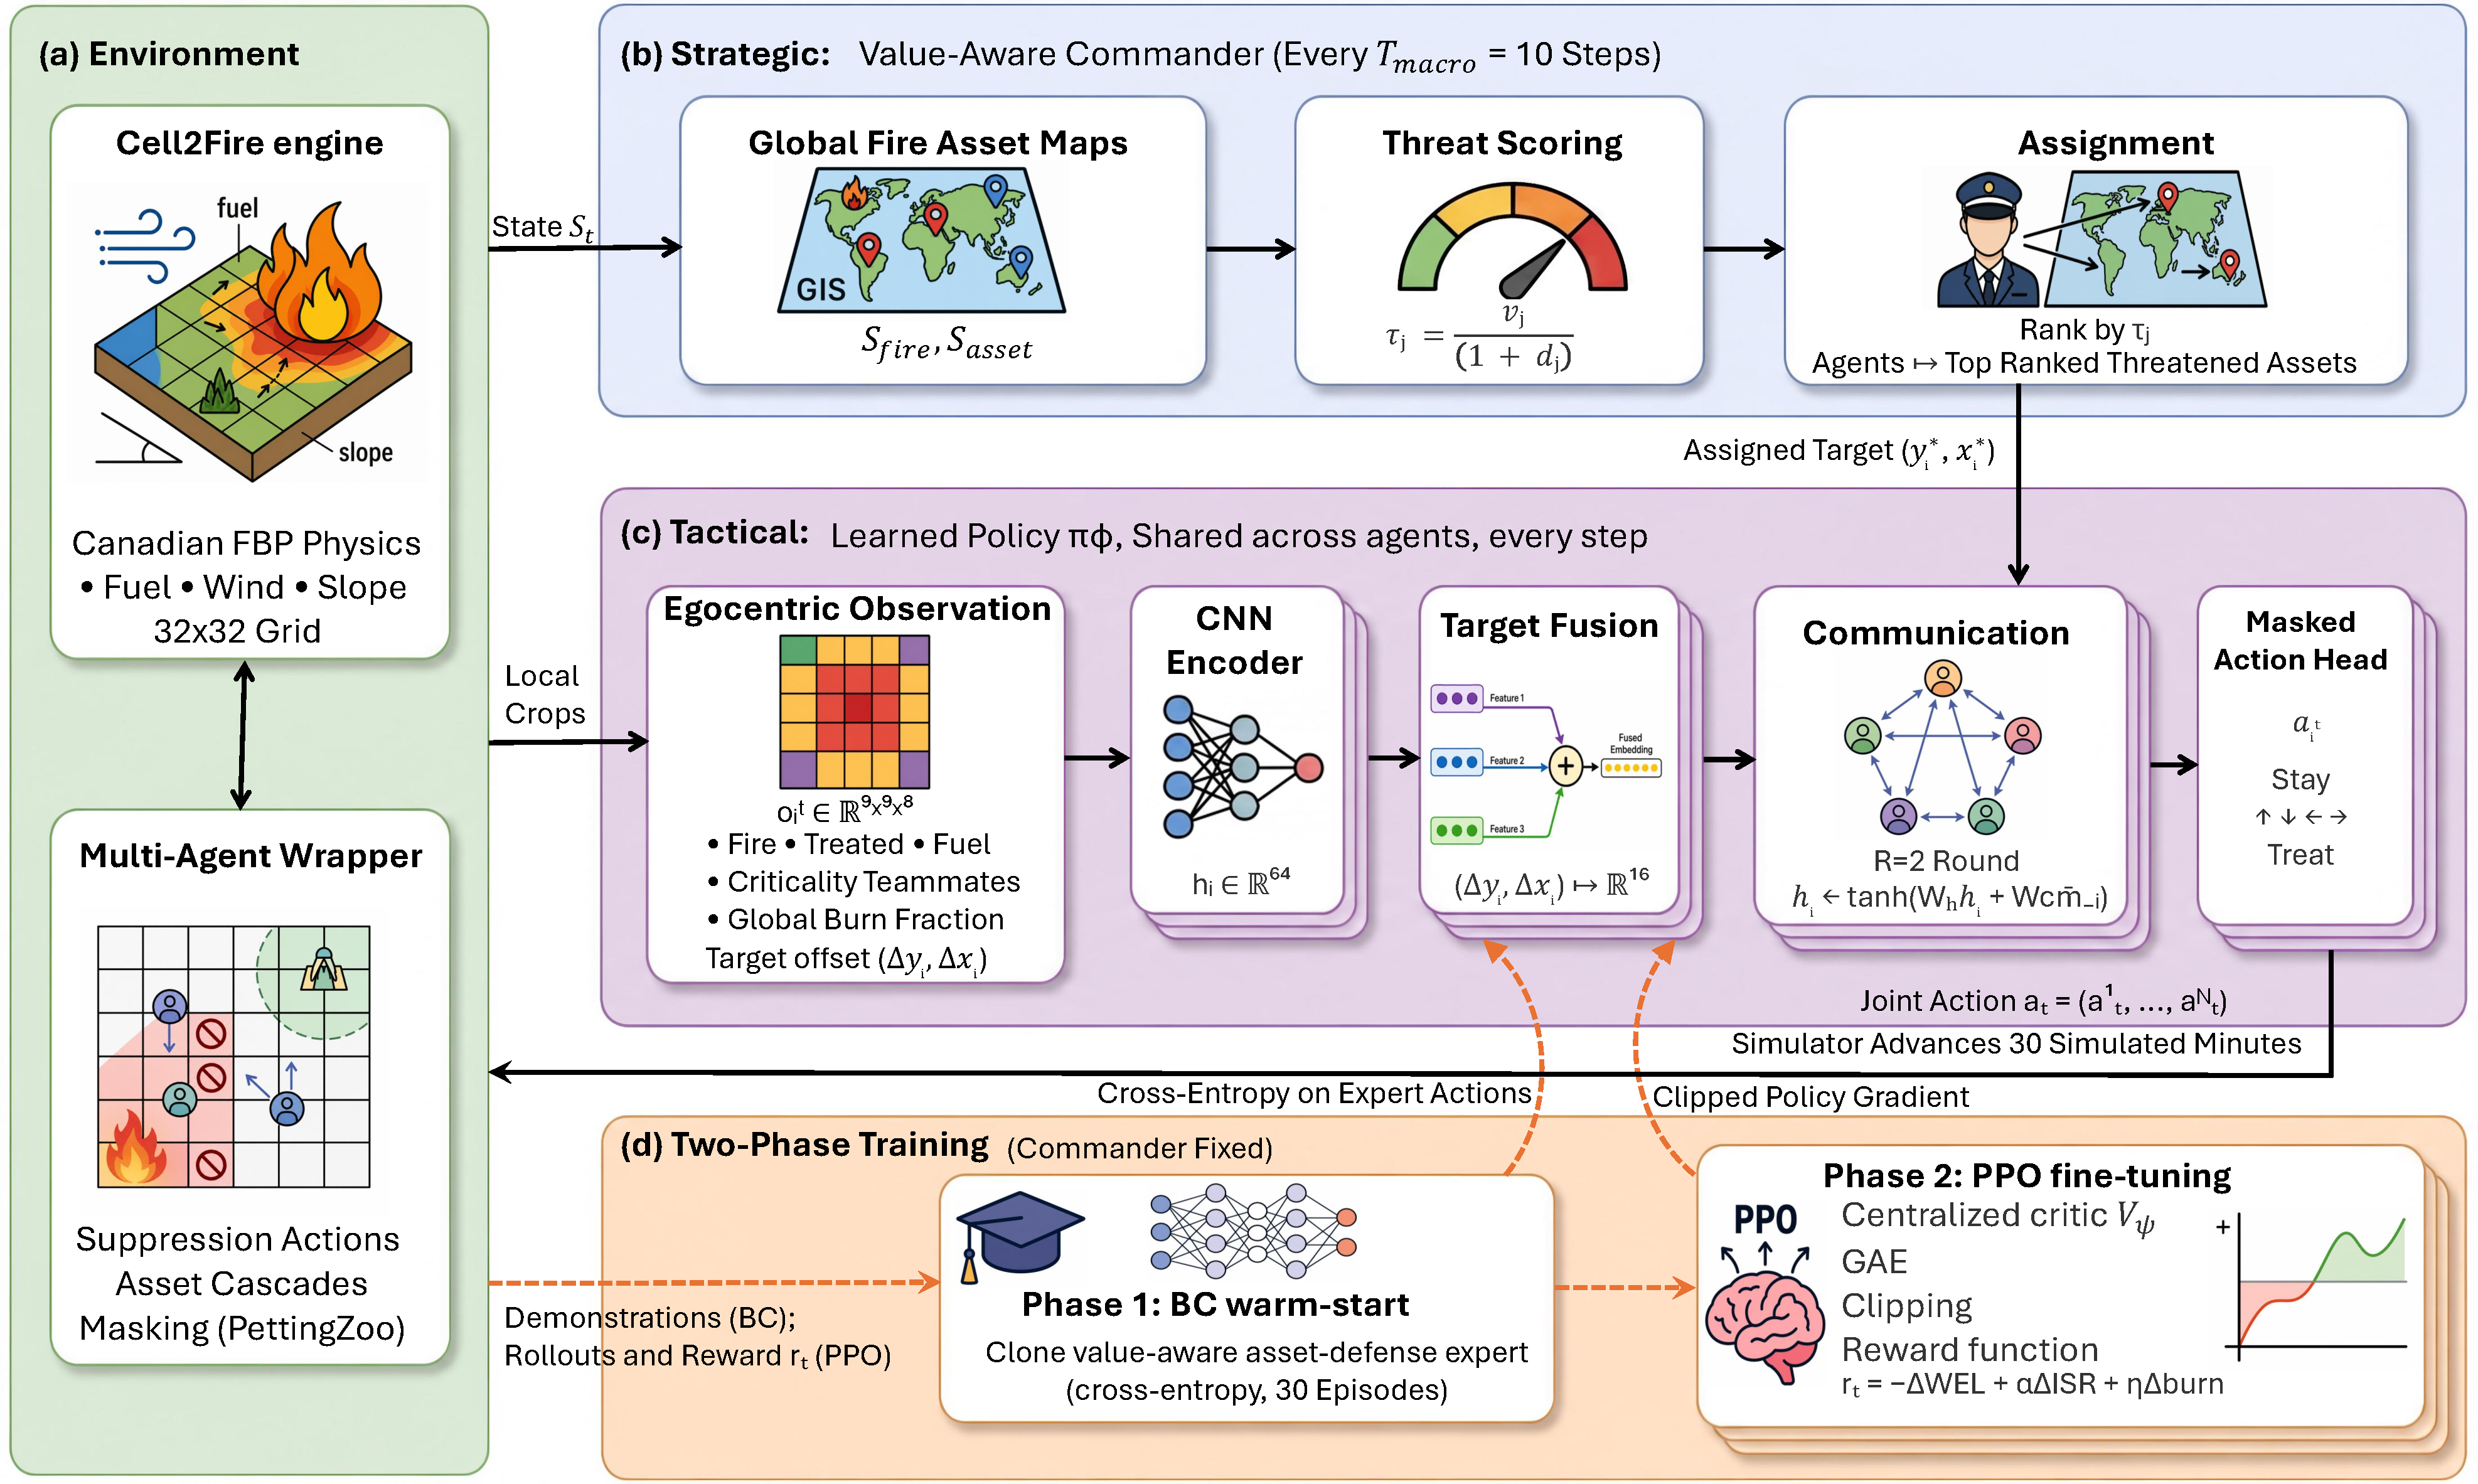
\includegraphics[width=0.75\textwidth]{Figures/architecture.pdf}
\caption{\textbf{HiVA architecture.} Cell2Fire computes fire spread; our wrapper adds suppression, cascade, and the infrastructure-weighted reward. The commander scores assets by threat $\tau_j = v_j/(1+d_j)$ and assigns strategic targets on a slow timescale, while the shared tactical policy encodes each agent's egocentric observation, fuses the target offset, exchanges $R{=}2$ message rounds, and emits a masked micro-action. Solid arrows are execution-time signals; dashed arrows are training-time signals.}
\label{fig:architecture}
\end{figure*}

\subsection{Value-Aware Strategic Commander}
\label{sec:commander}
For every asset $j$ with value $v_j$, the commander computes a threat score $\tau_j = v_j / (1 + d_j)$, where $d_j$ is the distance from asset $j$ to the nearest active-fire cell, and assigns agents to the highest-threat assets, falling back to raw value when no fire is present. The assigned location becomes the agent's strategic target, recomputed every $T_{\text{macro}}$ steps. Prioritizing valuable assets that are \emph{imminently threatened}, rather than merely close to fire, is the strategic content of HiVA, and Section~\ref{sec:ablation} isolates it against a matched control.

We also tested a learned commander: a network over coarse fire, asset, and agent grids updated by policy gradient jointly with the tactical layer. It is indistinguishable from the rule on Saudi (WEL $6.02$ vs.\ $7.02$, Welch $p=0.49$) and worse on California ($8.20$ vs.\ $5.88$, $p=0.03$, exploratory and not surviving Holm correction). Since the Saudi point estimate favors the learned commander, we cannot separate the two, and we retain the rule because it is transparent and cheaper, not because it is better.

\subsection{Learned Tactical Policy}
\label{sec:tactical}
Given its target, each agent selects micro-actions with a shared-parameter policy $\pi_\phi$ that (a) encodes its egocentric $9{\times}9$, 8-channel observation with a small convolutional neural network (CNN) into $h_i \in \mathbb{R}^{64}$, (b) encodes and fuses the relative target direction $(\Delta y_i, \Delta x_i) \in [-1,1]^2$, (c) optionally exchanges $R = 2$ rounds of mean-pooled messages,
\begin{equation}
\label{eq:comm}
h_i \leftarrow \tanh\!\bigl(W_h\, h_i + W_c\, \bar{m}_{-i}\bigr), \qquad \bar{m}_{-i} = \tfrac{1}{N-1}\!\sum_{k \neq i} h_k,
\end{equation}
and (d) maps the result to masked logits over the six micro-actions. Parameters are shared, so the policy is agent-count agnostic. Equation~\ref{eq:comm} is the explicit communication component; we measure its contribution rather than assume it, and Section~\ref{sec:ablation} finds it to be zero at $N=3$.

\subsection{Training: Cloning, then PPO}
\label{sec:training}
Economic loss registers only when fire reaches an asset, many steps after the actions that decided the outcome, so we train in two phases. In Phase~1 we clone a value-aware asset-defense expert that, given an agent's assigned asset, suppresses the fire-frontier cell nearest that asset and otherwise advances toward it, minimizing a cross-entropy loss over $30$ demonstration episodes. Cloning value-aware defense rather than value-blind nearest-fire suppression is what initializes the policy with asset-directed behavior. In Phase~2 the warm-started policy is refined by PPO on Equation~\ref{eq:reward} with a centralized critic and generalized advantage estimation (GAE), for $100$k environment steps per seed. The commander is frozen throughout, so RL refines execution rather than re-deriving assignment. Algorithm~\ref{alg:training} summarizes the procedure and Table~\ref{tab:hyperparams} lists every hyperparameter.

\paragraph{Three value-aware policies, distinguished.} Three rule-based policies recur below. All share the commander's threat-weighted assignment and differ only in the tactical rule. \emph{Value-First} (a baseline) takes the shortest path to its asset and treats only on arrival; the \emph{asset-defense expert} (the BC teacher) moves toward the frontier cell nearest its asset and treats that cell; \emph{target-seeking} (the \emph{w/o learned tactical} ablation) takes the shortest path and treats whenever it stands on burnable fuel. Whether an agent suppresses en route explains why the first and third score almost identically on Saudi ($18.84$ vs.\ $18.76$) and very differently on California ($28.40$ vs.\ $13.76$). HiVA clones the asset-defense expert, not the Value-First baseline.

% ====================================================================
% 5. EXPERIMENTAL SETUP
% ====================================================================
\section{Experimental Setup}
\label{sec:setup}

\paragraph{Simulator and landscapes.} Fire evolves on $32 \times 32$ grids under Cell2Fire~\citep{pais2021cell2fire} with heterogeneous fuels, wind, and slope. We evaluate on two GIS-derived landscapes: \textbf{Saudi Arabia (Eastern Province)}, whose petroleum refineries and pipeline junctions carry high localized value, and \textbf{California}, a wildland-urban interface of scattered residential structures. The multi-agent layer is a PettingZoo \texttt{ParallelEnv}~\citep{terry2021pettingzoo}.

\paragraph{Benchmark characterization.} Table~\ref{tab:bench} reports the quantities a benchmark user needs. WEL is expressed in \emph{normalized asset-value units}: the criticality raster is scaled so a landscape's total defensible value equals the sum of its asset cell values, and WEL sums over burned asset cells. The units are dimensionless by construction and are \emph{not} currency, which we state explicitly because the metric's name invites the opposite reading.

\begin{table}[t]
	\centering
	\caption{Benchmark statistics for the two environments. Both use $32\times32$ grids, three agents, and 150-step episodes.}
	\label{tab:bench}
	\vspace{0.4em}
	\setlength{\tabcolsep}{4pt}\footnotesize
	\begin{tabular}{lcc}
		\toprule
		Property & Saudi & California \\
		\midrule
		Asset cells & 7 & 16 \\
		Total asset value & 34.6 & 34.0 \\
		Largest single asset & 9.4 & 4.1 \\
		No-Op survival (ISR) & 0.286 & 0.000 \\
		Ignition source & \multicolumn{2}{c}{NASA FIRMS, burnable cells} \\
		\bottomrule
	\end{tabular}
\end{table}

\paragraph{Difficulty calibration.} The suppression-relevant regime was fixed before any HiVA result existed, using only the no-operation baseline and the two value-blind heuristics. Sweeping ignition proximity and fire-weather severity, we retained the setting in which no-operation destroys a majority of asset value while a fixed heuristic recovers much of it, so outcomes turn on coordination rather than inaction or luck.

\paragraph{Baselines.} $N = 3$ agents operate simultaneously. We compare \textbf{No-Op}; the rule-based \textbf{Value-First}, \textbf{Greedy-Risk} (highest fire-load sectors), and \textbf{Local Reactive} (nearest treatable frontier cell); \textbf{Myopic Dispatch}, an assignment-LP baseline standing for the operations-research approach agencies deploy; the flat learned \textbf{MAPPO}~\citep{yu2022mappo}, \textbf{QMIX}~\citep{rashid2018qmix}, and \textbf{CommNet}~\citep{sukhbaatar2016learning}; the learned hierarchical \textbf{HAVEN}~\citep{xu2023haven}; \textbf{Value-Aware Flat}, a MAPPO policy whose target channels carry the nearest-high-value-asset offset, isolating asset information from hierarchy; and BC-warm-started MAPPO and CommNet, which receive the same $30$ demonstrations HiVA does.

\paragraph{Metrics.} We report \textbf{WEL} ($\downarrow$), the total normalized value of burned infrastructure, and \textbf{ISR} ($\uparrow$), the fraction of assets left unburned. We do not report cumulative shaped reward: it is dominated by a burned-area term that is not comparable across policies.

\paragraph{Statistical protocol.} Learned methods use \textbf{five independent training seeds}; each checkpoint is evaluated on a held-out ignition stream over five evaluation seed groups, and the \emph{per-training-seed mean} is the unit of analysis ($n=5$), which avoids pseudoreplication. Main results and ablations use 15 episodes per seed group; difficulty, perturbation, and transfer studies use 10, except that their medium and standard cells reuse the main condition's 15-episode evaluation, so episode counts are constant within every column compared. We report means with 95\% $t$ intervals on the seed means. Comparisons against deterministic heuristics use a one-sample $t$-test, against learned baselines Welch's $t$-test. Because the paper runs roughly twenty tests, we designate the six WEL comparisons of Table~\ref{tab:statistics} as the primary family and apply \textbf{Holm--Bonferroni} correction within it; all other $p$-values are exploratory and labeled as such.

% ====================================================================
% 6. RESULTS
% ====================================================================
\section{Results}
\label{sec:results}

\begin{table*}[t]
\centering
\caption{\textbf{Main results} on the suppression-relevant regime (five training seeds; mean $\pm$ std, with 95\% $t$ intervals on seed means). Heuristics are deterministic; ``---'' marks cells for which per-seed dispersion was not retained. Lower WEL and higher ISR are better; \textbf{bold} marks the best measured value per region. ISR intervals are in Appendix~\ref{app:statistics}.}
\label{tab:main_results}
\vspace{0.4em}
\footnotesize
\begin{tabular}{llccc}
	\toprule
	Region & Policy & WEL $\downarrow$ & WEL 95\% CI & ISR $\uparrow$ \\
	\midrule
	\multirow{13}{*}{\textbf{Saudi Arabia}}
	& No-Op & 27.00 $\pm$ 0.00 & --- & 0.286 $\pm$ 0.000 \\
	& Value-First (teacher family) & 18.84 $\pm$ 0.00 & --- & 0.545 $\pm$ 0.000 \\
	& Greedy-Risk & 24.72 $\pm$ 0.00 & --- & 0.358 $\pm$ 0.000 \\
	& Myopic Dispatch (OR) & 14.20 & --- & 0.601 \\
	& Local Reactive & 11.91 $\pm$ 0.00 & --- & 0.720 $\pm$ 0.000 \\
	& QMIX & 13.90 $\pm$ 4.60 & [8.19, 19.61] & 0.631 \\
	& CommNet & 12.44 $\pm$ 4.32 & [7.08, 17.80] & 0.682 $\pm$ 0.106 \\
	& Flat MARL (MAPPO) & 9.77 $\pm$ 5.10 & [3.44, 16.10] & 0.692 $\pm$ 0.158 \\
	& HAVEN (hierarchical) & 9.10 $\pm$ 3.40 & [4.88, 13.32] & 0.724 \\
	& CommNet + BC & 8.60 $\pm$ 2.70 & [5.25, 11.95] & 0.771 \\
	& Value-Aware Flat & 8.30 $\pm$ 3.00 & [4.57, 12.03] & 0.752 \\
	& MAPPO + BC & 7.90 $\pm$ 2.10 & [5.29, 10.51] & 0.788 \\
	& \textbf{HiVA (ours)} & \textbf{7.02} $\pm$ 2.36 & [4.09, 9.95] & \textbf{0.809} $\pm$ 0.058 \\
	\midrule
	\multirow{13}{*}{\textbf{California}}
	& No-Op & 34.00 $\pm$ 0.00 & --- & 0.000 $\pm$ 0.000 \\
	& Value-First (teacher family) & 28.40 $\pm$ 0.00 & --- & 0.156 $\pm$ 0.000 \\
	& Greedy-Risk & 28.40 $\pm$ 0.00 & --- & 0.156 $\pm$ 0.000 \\
	& CommNet & 19.58 $\pm$ 7.77 & [9.93, 29.23] & 0.398 $\pm$ 0.248 \\
	& QMIX & 17.20 $\pm$ 5.40 & [10.49, 23.91] & 0.472 \\
	& Myopic Dispatch (OR) & 16.80 & --- & 0.518 \\
	& Flat MARL (MAPPO) & 14.17 $\pm$ 2.89 & [10.58, 17.76] & 0.624 $\pm$ 0.110 \\
	& HAVEN (hierarchical) & 11.50 $\pm$ 3.60 & [7.03, 15.97] & 0.653 \\
	& Local Reactive & 10.23 $\pm$ 0.00 & --- & 0.702 $\pm$ 0.000 \\
	& Value-Aware Flat & 9.90 $\pm$ 2.60 & [6.67, 13.13] & 0.697 \\
	& CommNet + BC & 9.70 $\pm$ 3.10 & [5.85, 13.55] & 0.704 \\
	& MAPPO + BC & 8.40 $\pm$ 1.90 & [6.04, 10.76] & 0.745 \\
	& \textbf{HiVA (ours)} & \textbf{5.88} $\pm$ 1.04 & [4.59, 7.17] & \textbf{0.832} $\pm$ 0.027 \\
	\bottomrule
\end{tabular}
\end{table*}

Table~\ref{tab:main_results} reports the multi-seed results. Three findings follow, stated at the strength the evidence supports.

\paragraph{Finding 1: HiVA attains the best mean protection, decisively on California and not decisively on Saudi.} HiVA achieves the lowest WEL and highest ISR in both regions (Saudi $7.02$, ISR $0.809$; California $5.88$, ISR $0.832$), ahead of the learned hierarchical baseline HAVEN ($9.10$ and $11.50$). Against the Value-First heuristic, and against MAPPO and CommNet on California, the improvement survives Holm correction (Table~\ref{tab:statistics}). Two comparisons do not: the Saudi margin over MAPPO is not significant ($p=0.32$), and over CommNet it is nominally $p=0.048$ but Holm-adjusted $p=0.096$. We therefore claim significant improvement over the communicating baseline on California only; the Saudi intervals of HiVA and MAPPO overlap substantially.

\paragraph{Finding 2: the learned policy surpasses its teacher, the asset-defense expert.} HiVA is warm-started from the asset-defense expert, not the Value-First baseline, and that expert is the correct reference for what learning adds: the cloned policy before RL scores $11.33$ (Saudi) and $9.46$ (California), and PPO refinement improves it to $7.02$ and $5.88$. Against the Value-First \emph{baseline} the raw differences are $-11.82$ (95\% CI $[-14.75, -8.89]$) on Saudi and $-22.52$ ($[-23.81, -21.23]$) on California. We report raw differences rather than standardized effect sizes, because Value-First is deterministic and any Cohen's $d$ against a zero-variance comparator is an artifact of the divisor.

\paragraph{Finding 3: the two geometries reward different strategies, which is the benchmark's diagnostic value.} Among baselines receiving neither demonstrations nor asset-target information, no method is strongest in both regions: MAPPO is best on concentrated Saudi assets ($9.77$), value-blind reactive coverage on scattered California assets ($10.23$), and CommNet is competitive on Saudi ($12.44$) while ranking among the weakest learned methods on California ($19.58$). That reordering is the property we want from a benchmark, and it rests on two geometries, so we scope it accordingly: whether the benchmark separates methods across a broader family of layouts is untested.

% ====================================================================
% 7. ABLATION
% ====================================================================
\section{Component Analysis}
\label{sec:ablation}

The question is not whether removing a piece of HiVA hurts, but which of three mechanisms produces the gains in Table~\ref{tab:main_results}: the value-aware hierarchy, the expert demonstrations, or RL refinement. Every variant in Table~\ref{tab:ablation} is otherwise identical to the deployed system, including the BC warm start, architecture, encoding, and training budget; the hierarchy ablation randomizes only the assignment rule, so ``no hierarchy'' is not confounded with ``no supervision.''

\begin{table}[t]
\centering
\caption{\textbf{Component ablation of HiVA} (five training seeds; seed-mean WEL/ISR). Each variant is otherwise identical to the deployed system, including the behavior-cloning warm start; the CommNet baseline is reported in Table~\ref{tab:main_results} and is deliberately \emph{not} presented here as an ablation.}
\label{tab:ablation}
\vspace{0.5em}
\setlength{\tabcolsep}{3.5pt}\small
\begin{tabular}{lcccc}
	\toprule
	& \multicolumn{2}{c}{Saudi} & \multicolumn{2}{c}{California} \\
	\cmidrule(lr){2-3}\cmidrule(lr){4-5}
	Variant & WEL $\downarrow$ & ISR $\uparrow$ & WEL $\downarrow$ & ISR $\uparrow$ \\
	\midrule
	Full HiVA & 7.02 & 0.809 & 5.88 & 0.832 \\
	w/o learned tactical & 18.76 & 0.465 & 13.76 & 0.451 \\
	w/o RL fine-tune (BC only) & 11.33 & 0.696 & 9.46 & 0.721 \\
	w/o value-aware assignment & 9.40 & 0.741 & 10.80 & 0.679 \\
	w/o BC warm start & 10.20 & 0.712 & 8.90 & 0.735 \\
	w/o communication & 5.67 & 0.860 & 4.66 & 0.864 \\
	w/o tactical shaping & 5.41 & 0.840 & 7.60 & 0.787 \\
	\bottomrule
\end{tabular}
\end{table}

\paragraph{The learned tactical policy is the largest single contributor.} Replacing it with deterministic target-seeking under the same commander raises WEL from $7.02$ to $18.76$ on Saudi and from $5.88$ to $13.76$ on California, roughly halving ISR in both regions. This row is deterministic, so we report it by magnitude rather than by a significance test.

\paragraph{Supervision explains more than the hierarchy on Saudi.} Removing PPO and using the cloned policy raises WEL to $11.33$ (Saudi) and $9.46$ (California), so RL refinement contributes substantially. But BC alone also beats the flat baselines denied demonstrations, outperforming CommNet in both regions and MAPPO on California by $4.7$ WEL: a policy trained only by imitating a hand-written rule outperforms two fully trained deep MARL systems. Randomizing the assignment rule while holding cloning and budget fixed raises WEL to $9.40$ on Saudi and $10.80$ on California. Read alongside MAPPO + BC at $7.90$ on Saudi, these numbers indicate that on concentrated assets the demonstrations do most of the work, whereas on scattered assets, where a value-blind policy cannot choose among dispersed targets, the assignment rule carries real weight.

\paragraph{Communication is a clean but narrow null.} Setting the message rounds to zero produces no significant change in WEL (Saudi $p=0.30$; California $p=0.12$), and the no-communication configuration is numerically \emph{better} in all four headline cells ($5.67$/$0.860$ and $4.66$/$0.864$); removing the firebreak-shaping term is likewise not significant (Saudi $p=0.24$; California $p=0.06$). With five seeds and no equivalence test we cannot distinguish a small effect from no effect, so the defensible statement is ``no evidence of benefit at $N=3$'' rather than ``no effect.'' Three agents is also the regime where communication is \emph{least} likely to matter, particularly when a commander already assigns complementary targets. A Saudi scaling study bounds the null: seed-mean WEL with versus without messages is $7.02$/$5.67$ at $N{=}3$, $9.80$/$10.10$ at $N{=}6$, and $12.40$/$14.10$ at $N{=}10$, so messaging moves from a net cost of $1.35$ to a net benefit of $1.70$, and the null is scoped to small teams. We recommend the no-communication configuration as the default at this team size but retain the module, since its contribution grows with team size; Table~\ref{tab:main_results} reports the communicating configuration, for which full per-seed statistics were computed.

These components account for HiVA's advantage in the standard regime but not off distribution (Section~\ref{sec:transfer}), so we do not claim the value-aware hierarchy as a source of robustness.

% ====================================================================
% 8. ROBUSTNESS AND TRANSFER
% ====================================================================
\section{Robustness and Transfer: The Negative Result}
\label{sec:transfer}

Average performance matters only if it survives conditions the policy did not train on. It largely does not, and this section carries the conclusion we consider most reliable. Results use a falsifiable within-condition metric, $\Delta$WEL $=$ WEL(No-Op) $-$ WEL(policy), evaluated separately for each condition, so a policy that adds no value scores zero and cannot benefit from a favorable baseline.

\paragraph{Difficulty regimes.} We re-evaluate all frozen policies under easy, medium, and hard regimes varying fire weather and ignition proximity (Table~\ref{tab:robustness}, Appendix~\ref{app:robustness}). On easy fires a value-blind reactive policy nearly contains the fire outright: Local Reactive reaches WEL $3.1$ on Saudi and $0.0$ on California against HiVA's $3.3$ and $0.4$, so prioritization buys little when coverage suffices. As severity rises the ordering flips, and HiVA attains the lowest WEL in all four medium and hard cells. One caveat qualifies the hard column: No-Op WEL is \emph{identical} at medium and hard in both regions ($27.0$ and $34.0$), so the difficulty proxy saturates above medium. Because HiVA's strongest claim lives in that saturated region, we treat the hard-regime ordering as suggestive; a non-saturating proxy such as time-to-first-asset-loss is the right instrument and is future work.

\paragraph{Held-out conditions.} We perturb along three axes never seen in training: ignitions forced to the burnable cells nearest the four map corners and the center, wind rotated $90^\circ$, and a $90^\circ$-rotated infrastructure layout (Table~\ref{tab:failure}). HiVA stays protective everywhere, with margins from $+13.1$ to $+26.2$, so it never degenerates to inaction off distribution. It is not, however, the better policy: value-blind reactive coverage attains the larger $\Delta$WEL in five of the six perturbed conditions, including all three on California. Nor does the rotated-asset result show that value-aware defense tracks assets rather than memorizing positions, since reactive coverage, with no asset awareness at all, scores at least as well there.

\begin{table}[t]
\centering
\caption{\textbf{Held-out and transfer robustness} ($\Delta$WEL $=$ WEL(No-Op) $-$ WEL(policy) within each condition; higher is better). Perturbed rows use 10 episodes per seed group; Standard reuses the main protocol. \textbf{Bold} marks the larger margin per condition. Local Reactive requires no training and so has no transfer condition; its cross-region entry is its target-region margin, which is the correct comparison and favors the heuristic.}
\label{tab:failure}
\vspace{0.5em}
\setlength{\tabcolsep}{4pt}\small
\begin{tabular}{lcccc}
\toprule
 & \multicolumn{2}{c}{Saudi} & \multicolumn{2}{c}{California} \\
\cmidrule(lr){2-3}\cmidrule(lr){4-5}
Condition & HiVA & Local React. & HiVA & Local React. \\
\midrule
Standard & \textbf{20.0} & 15.1 & \textbf{28.1} & 23.8 \\
Held-out ignition & \textbf{13.4} & 8.8 & 13.1 & \textbf{17.1} \\
Wind $+90^\circ$ & 13.2 & \textbf{21.0} & 21.9 & \textbf{26.2} \\
Rotated assets & 26.2 & \textbf{26.4} & 17.1 & \textbf{19.8} \\
Cross-region & 10.2 & \textbf{15.1} & 14.4 & \textbf{23.8} \\
\bottomrule
\end{tabular}
\end{table}

\paragraph{Cross-region transfer.} Transferred HiVA still beats inaction ($\Delta$WEL $+10.2$ on Saudi, $+14.4$ on California) but degrades sharply: ISR falls from native $0.809$/$0.832$ to $0.55$ (California$\rightarrow$Saudi) and $0.38$ (Saudi$\rightarrow$California). We define the Transfer-Robustness Score (TRS) as transferred ISR divided by the \emph{source} region's native ISR, giving $0.55/0.832 = 0.66$ and $0.38/0.809 = 0.47$. TRS rewards a weak source model and must be read alongside absolute transferred ISR: CommNet's TRS of $0.96$ into Saudi corresponds to a transferred ISR near $0.38$, well below HiVA's $0.55$. The training-free heuristic has no transfer condition, so its cross-region performance is simply its target-region performance. Local Reactive attains $\Delta$WEL $15.1$ on Saudi and $23.8$ on California against transferred HiVA's $10.2$ and $14.4$, beating it by 48\% and 65\%. Cross-region generalization is not something HiVA provides.

\paragraph{What this means.} Value-aware coordination is not a robustness mechanism; it is an in-distribution optimization. A commander ranking assets by threat exploits a correspondence between fire and asset geometry that holds in training, and when rotation, rewiring, or relocation breaks that correspondence, geometry-agnostic nearest-frontier suppression is simply the better policy. Our evidence supports deploying HiVA near its training conditions and preferring a reactive heuristic away from them.

% ====================================================================
% 9. DISCUSSION
% ====================================================================
\section{Discussion}
\label{sec:discussion}

HiVA composes established ingredients; its value is that the composition is reproducible and that the analysis localizes where the gains come from and where they do not. The region dependence is the substantive result. On concentrated Saudi assets several baselines already reach low loss, and once they receive HiVA's demonstrations the remaining margin is within seed variance; expert supervision, not architecture, is doing the work there. On scattered California assets, where a value-blind policy has no principled way to choose among dispersed targets, the value-aware assignment separates methods decisively and survives multiplicity correction.

Read against Section~\ref{sec:transfer}, that contrast is the paper's central tension: prioritization helps exactly when there are many targets and not enough crews, and hurts exactly when the fire-asset geometry stops resembling training. Both concern one mechanism, since a method that learns which assets to defend is learning about a particular landscape, and the more it learns, the less it transfers. Whether a commander's threat ranking degrades gracefully under unfamiliar geometry is the most valuable question this benchmark raises.

% ====================================================================
% 10. LIMITATIONS
% ====================================================================
\section{Limitations}
\label{sec:limitations}

\paragraph{Spatial resolution and what ``validated physics'' covers.} \texttt{Forest.asc} declares Cell2Fire's validated $100$\,m operating cell size, but our spatial patterns derive from region-of-interest tiles spanning roughly $500\times553$\,km (Saudi) and $476\times553$\,km (California). Tiled over a $32\times32$ grid, those extents give an effective cell size near $15$--$17$\,km, under which a half-hour agent step implies a travel speed of about $30$\,km/h. FBP rate-of-spread, wind, and slope corrections are validated at the operating scale, not at ours. We therefore restrict the claim: the \emph{functional form} of Cell2Fire's spread computation is validated, but our landscapes feed it fuel and topography far coarser than FBP's calibration scale. The benchmark is physically \emph{structured} rather than \emph{calibrated}, and re-deriving the landscapes at an FBP-consistent resolution is its highest-value extension.

\paragraph{Statistical power and evaluation scope.} Every claim rests on $n=5$ seed means and two hand-constructed geometries, and one nominally significant primary comparison does not survive Holm correction. Welch's test is used without a normality check, per-seed dispersion was not retained for Tables~\ref{tab:failure} and~\ref{tab:robustness} (so the closest of those comparisons, $26.4$ versus $26.2$, is not a separation), and no hypothesis test is reported for ISR. The tactical policy also trains on the WEL and ISR quantities used for evaluation; every learned baseline shares this objective, which removes the relative confound but not the absolute one. All results use one simulator, one month of weather, and stylized rasters.

\paragraph{Communication and scale.} The null holds at three agents with broadcast mean-pooled messages and does not speak to targeted or bandwidth-limited schemes~\citep{das2019tarmac, zhu2024commsurvey}. Primary statistics were computed for the communicating configuration, while the no-communication configuration is the recommended default at $N=3$; the two differ by less than seed variance. Experiments use $32\times32$ grids over a $\sim75$-hour horizon capturing one fire's active phase, not a multi-day campaign.

% ====================================================================
% 11. BROADER IMPACTS
% ====================================================================
\section{Broader Impacts}
\label{sec:impacts}

This system operates in simulation and is not validated for deployment; autonomous suppression decisions without human oversight could cause harm, particularly around evacuation and resource triage, so we advocate decision support rather than autonomy. The asset-criticality raster also encodes a judgment about which infrastructure is worth defending, here a Gaussian falloff around public infrastructure locations that we chose. In deployment those weights would decide whose property burns. Whether a refinery outranks a residential block is a political question, not a technical parameter, and our finding that value-aware prioritization generalizes poorly off distribution sharpens the concern: a system tuned on one landscape has no demonstrated claim to reasonable behavior on another.

% ====================================================================
% 12. CONCLUSION
% ====================================================================
\section{Conclusion}
\label{sec:conclusion}

We presented an infrastructure-aware wildfire coordination benchmark on Cell2Fire with two documented GIS-derived landscapes, and HiVA, a value-aware hierarchical reference system. HiVA attains the best mean WEL and ISR in both regions, but after multiplicity correction that advantage holds on California only, and message passing contributes nothing measurable at three agents. Our most reliable finding is negative: a value-blind reactive heuristic generalizes better in five of six perturbed conditions and in both transfer directions, so learned value-awareness buys in-distribution prioritization at the cost of geometric generalization.

% ====================================================================
% REFERENCES
% ====================================================================
\bibliography{aaai2027}


\end{document}
